\documentclass[UTF8]{ctexart}
\usepackage{amsmath,empheq,graphicx,float,subfigure,
amssymb,geometry,tikz,enumitem,svg}

\geometry{a4paper,left=1cm,right=1cm,top=1.2cm,bottom=1.2cm}
\ctexset{section={number=\chinese{section},name={,、}},
subsubsection={name={,、}},
subsection={number=\chinese{subsection},name={(,)}}}
\renewcommand{\thesubsubsection}{\arabic{subsubsection}}

\newcommand*\circled[1]{\tikz[baseline=(char.base)]{
            \node[shape=circle,draw,inner sep=1.5pt] (char) {#1};}}
\counterwithout*{subsubsection}{subsection}

\begin{document}
\title{2019年普通高等学校招生全国统一考试
    (课标全国卷\uppercase\expandafter{\romannumeral3}).\\
    \textbf{理数}}
\author{Wang}
\maketitle

\section{选择题}

\subsubsection{已知集合$A=\{-1,0,1,2\},B=\{x|x^2\leq 1\}$,则$A\cap B=$\hfill (\qquad)}
$A.\{-1,0,1\}\hfill B.\{1,0\}\hfill C.\{-1,1\}\hfill D.\{0,1,2\}$

\subsubsection{若$z(1+i)=2i$,则$z=$\hfill (\qquad)}
$A. -1-i\hfill B. -1+i\hfill C. 1-i\hfill D. 1+i$

\subsubsection{《西游记》《三国演义》《水浒传》和《红楼梦》是中国古典文学瑰宝,
    并称为中国古典小说四大名著.某中学为了了解本校学生阅读四大名著的情况,随机调查
    了100位学生,其中阅读过《西游记》或《红楼梦》的学生共有90位,阅读过《红楼梦》
    的学生共有80位,阅读过《西游记》且阅读过《红楼梦》的学生共有60位,则该校阅读过
    《西游记》的学生人数与该校学生总数比值的估计值为\hfill (\qquad)}
$A. 0.5\hfill B. 0.6\hfill C. 0.7\hfill D. 0.8$

\subsubsection{$(1+2x^2)(1+x^4)$的展开式中$x^3$的系数为\hfill (\qquad)}
$A. 12\hfill B. 16\hfill C. 20\hfill D. 24$

\subsubsection{已知各项均为正数的等比数列$\{a_n\}$的前4项和为15,
    且$a_5=3a_3+4a_1$,则$a_3=$\hfill (\qquad)}
$A. 16\hfill B. 8\hfill C. 4\hfill D. 2$

\subsubsection{已知曲线$y=ae^x+xlnx$在点$(1,ae)$处的切线方程为$y=2x+b$,则\hfill (\qquad)}
$A. a=e,b=-1 \hfill B. a=e,b=1\hfill C. a=e^{-1},b=1\hfill D. a=e^{-1},b=-1$

\subsubsection{函数$y=\frac{2x^3}{2^x+2^{-x}}$在$[-6,6]$的图像大致为\hfill (\qquad)}
\begin{figure}[H]
    \centering
    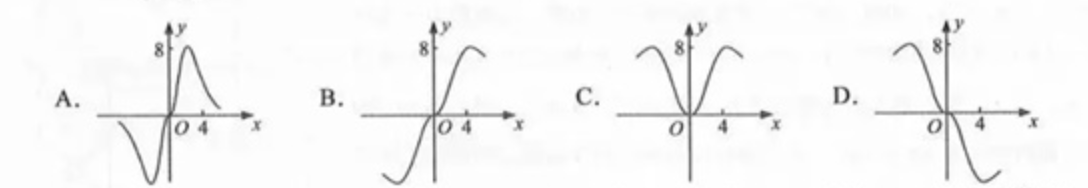
\includegraphics[width=1\textwidth]{pics/2019_3_7.png}
\end{figure}

\subsubsection{如图,点$N$为正方形$ABCD$的中心,$\triangle ECD$
    为正三角形,平面$ECD\perp$平面$ABCD,M$是线段ED的中点,则\hfill (\qquad)}
\begin{figure}[H]
    \centering
    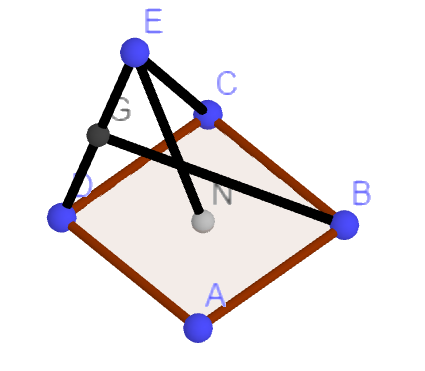
\includegraphics{pics/2019_3_8.png}
\end{figure}
$A. BM=EN$,且直线$BM,EN$是相交直线\hfill $B. BM\neq EN$,且直线$BM,EN$是相交直线\hfill \quad \par
$C. BM=EN$,且直线$BM,EN$是异面直线\hfill $D. BM\neq EN$,且直线$BM,EN$是异面直线\hfill \quad

\subsubsection{执行如图所示的程序框图,如果输入的$\epsilon$为0.01,则输入的s的值等于\hfill (\qquad)}
\begin{figure}[H]
    \centering
    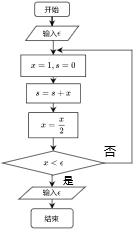
\includegraphics{pics/2019_3_9.png}
\end{figure}
$A. 2-\frac{1}{2^4}\hfill B. 2-\frac{1}{2^5}\hfill
    C. 2-\frac{1}{2^6}\hfill D. 2-\frac{1}{2^7}$

\subsubsection{双曲线$C:\frac{x^2}{4}-\frac{y^2}{2}=1$的右焦点为$F$,点$P$在$C$的
    一条渐近线上,$O$为坐标原点.若$|PO|=|PF|$,则$\triangle PFO$的面积为\hfill (\qquad)}
$A. \frac{3\sqrt{2}}{4}\hfill B. \frac{3\sqrt{2}}{2}\hfill
    C. 2\sqrt{2}\hfill D. 3\sqrt{2}$

\subsubsection{设$f(x)$是定义域为$R$的偶函数,且在$(0,+\infty)$单调递减,则\hfill (\qquad)}
$A. f(log_3\frac{1}{4})>f(2^{-\frac{3}{2}})>f(2^{-\frac{2}{3}})\hfill
    B. f(log_3\frac{1}{4})>f(2^{-\frac{3}{2}})>f(2^{-\frac{2}{3}})$\hfill \quad \par
$C. f(log_3\frac{1}{4})>f(2^{-\frac{3}{2}})>f(2^{-\frac{2}{3}})\hfill
    D. f(log_3\frac{1}{4})>f(2^{-\frac{3}{2}})>f(2^{-\frac{2}{3}})$\hfill \quad

\subsubsection{设函数$f(x)=\sin(\omega x+\frac{\pi}{5})(\omega>0)$已知$f(x)$
    在$[0,2\pi]$有且仅有5个零点.下述四个结论}

\begin{enumerate}[label=\protect\circled{\arabic*}]
    \item $f(x)$在$(0,2\pi)$有且仅有3个极大值点
    \item $f(x)$在$(0,2\pi)$有且仅有2个极小值点
    \item $f(x)$在$(0,\frac{\pi}{10})$单调递增
    \item $\omega$的取值范围是$[\frac{12}{5},\frac{29}{10})$
\end{enumerate}
其中所有正确的编号是\hfill (\qquad)\\
$A. \circled{1}\circled{4}\hfill B. \circled{2}\circled{3}\hfill
    C. \circled{1}\circled{2}\circled{3}\hfill D. \circled{1}\circled{3}\circled{4}$

\section{填空题}
\subsubsection{已知$\vec{a},\vec{b}$为单位向量,且$\vec{a}\cdot
        \vec{b}=0$,若$\vec{c}=2\vec{a}-\sqrt{5}\vec{b}$,则
    $\cos<\vec{a},\vec{c}> =\underline{\hbox to 15mm{}}.$}
\subsubsection{记$S_n$为等差数列$\{a_n\}$的前$n$项和,若$a_1\neq 0,a_2=3a_1$,则
    $\frac{S_{10}}{S_5}=$\underline{\hbox to 15mm{}}.}
\subsubsection{设$F_1,F_2$为椭圆$C:\frac{x^2}{36}+\frac{y^2}{20}=1$的两个焦点,$M$为$C$上一点
    且在第一象限,若$\triangle MF_1F_2$为等腰三角形,则$M$的坐标为\underline{\hbox to 15mm{}}.}
\subsubsection{学生到工厂劳动实践,利用3D打印技术制作模型.如图,该模型为长方体$ABCD-A_1B_1C_1D_1$挖
    去四棱锥$O—EFGH$后所得几何体,其中$O$为长方体的中心,$E,F,G,H$分别为所在棱的中点,$AB=BC=4c\quad m,
        AA_1=4\quad cm,$,3D打印所用原料密度为$0.9 g/cm^3$,不考虑打印损耗,制作该模型所需原料的质量为
    \underline{\hbox to 15mm{}}.}
\begin{figure}[htbp]
    \centering
    \includesvg{pics/2019_3_16.svg}
    \caption{svg image}
\end{figure}
\section{解答题}
\subsection{必考题}
\subsubsection{为了解甲、乙两种离子在小鼠体内的残留程度,进行如下试验:将200只小鼠随机分成$A,B$两组,
    每组100只,其中$A$组小鼠给服甲离子溶液,$B$组小鼠给服乙离子溶液.每只小鼠给服的溶液体积相同,摩尔浓度相
    同.经过一段时间后用某种科学方法测算出残留在小鼠体内离子的百分比.根据试验数据分别得到如下直方图:}
\end{document}
